\chapter{Strutture dei Sistemi Operativi}
Un sistema operativo mette a disposizione degli utenti (e dei loro programmi) molti servizi 
\begin{figure}[h]
    \centering
    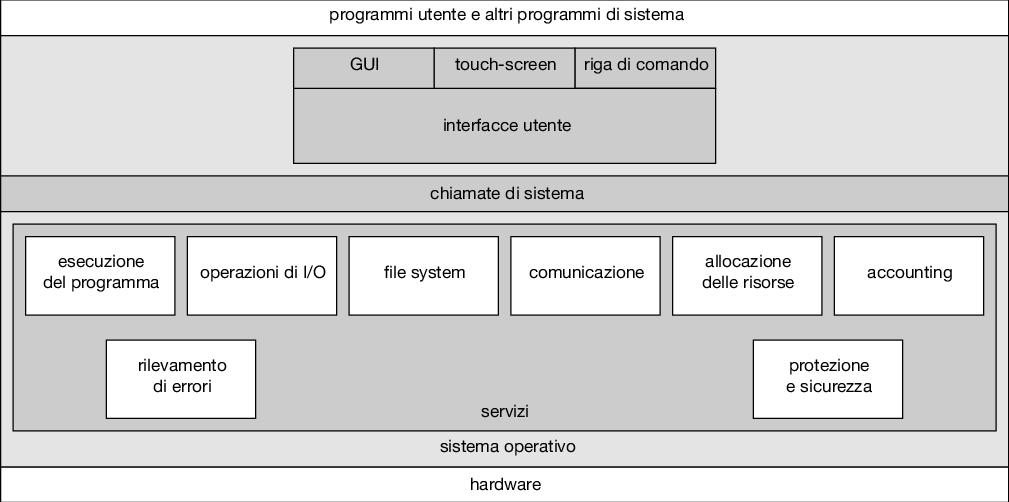
\includegraphics[width=0.5\linewidth]{images/Strutture-di-SO.png}
\end{figure}

Alcuni di questi servizi sono completamente invisibili agli utenti, altri sono parzialmente visibili, e altri sono direttamente usati dagli utenti.
Ma il \textit{grado di visibilità} dipende anche dal tipo di utente (Root, user, group)

\ex{Esempi di visibilità}{
\begin{itemize}
    \item Interfaccia col sistema operativo (terminale) (visibili)
    \item Chiamate di sistema (quasi sempre visibili)
    \item Gestione di processi (praticamente invisibili
\end{itemize}
}

\section{Interfaccia del Sistema Operativo}
L'interfaccia è lo strumento con il quale gli utenti interagiscono con il So, e ne sfruttano i servizi offerti.\\
Può essere un \textbf{interprete di comandi}, o un'\textbf{interfaccia grafica} con finestre e menù, ma di solito è possibile usare una combinazione di entrambi

\subsection{Interprete dei comandi}
Normalmente non fa parte del \textbf{kernel} SO; ma è un programma (o collezione di essi) fornito insieme al SO.\\
Un esempio d'interprete è la \textbf{shell} dell'MS-Dos oppure la \textbf{shell} Unix.\\
Una shell rimane semplicemente in attesa di ciò che l'utente scrive da linea di comando, ed ovviamente, esegue il comando stesso. Spesso, i comandi che possonoe ssere usati dagli utenti del SO sono dei semplici \textbf{eseguibili}. L'interprete si occupa di trovare sull'hard disk e lanciare il codice dell'eseguibile passando eventuali argomenti specificati.
\ex{Comando shell unix}{
\begin{enumerate}
    \item L'utente scrive \textit{rm myfile}
    \item l'interprete cerca un file eseguibile di nome "rm" e lo lancia, passandogli come parameteo "myfile"
\end{enumerate}
}
\nt{
Un comando utile può essere \textit{ps} che ti permette di vedere i processi attaccati alla tua shell
}

\section{Interfaccia grafica}
I moderni SO offrono anche una interfaccia grafica (GUI) per gli utenti, spesso più facile da imparare ed usare.\\
\textbf{Unix} offre varie interfaccie grafiche, sia proprietarie che open-source, come \textbf{KDE} e \textbf{GNOME}, e ogni utente del SO può scegliersi la sua

\section{Programmi/servizi di Sistema}
Non fanno parte del kernel del SO, ma vengono forniti insieme al SO, e rendono più facile, comodo e conveniente l’uso del Sistema.\\
Gli interpreti dei comandi e le interfacce grafiche sono gli esempi più evidenti di programmi di sistema. \\
Oltre a questi: editor, compilatori, browser, task manager etc etc.

\section{Chiamate di sistema (Syscall)}
Da ora in poi, chiameremo un programma in "esecuzione" come \textbf{processo}
Le system call costituiscono la vera e propria interfaccia tra i processi degli utenti e il Sistema Operativo.\\
Ad esempio, in Unix assumono la forma di procedure che possono essere inserite direttamente in programmi scritti con linguaggi ad alto livello (C, C++, …) \\
Sembra di usare una \textbf{subroutine}, ma l’esecuzione della system call trasferisce il controllo al SO, e in particolare alla porzione di codice del SO che implementa la particolare System Call invocata. \\
Ad esempio, in un programma C, per scrivere dentro ad un file:\\
\begin{lstlisting}[language=C]
fd = open("nomefile", O_WRONLY);
i = write(...)
close(fd)
\end{lstlisting}
\textbf{Open, write e close} sono delle syscall

\subsection{Chiamate di sistema: le "API"}
Application Programming Interface
Le API non sono ltro che uno strato intermedio tra le applicazione sviluppate dai programmatori e le syscall, per rendere più \textbf{facile} l'uso e migliorare la \textbf{portabilità} tra versioni.

\ex{Chiamate}{
Ad esempio, la libreria C dell’ambiente Unix è una semplice forma di API. In questa libreria esiste la funzione per aprire un file: \\
\textit{fopen}, \textit{fprintf} e \textit{fclose}
}

\section{Gestione dei processi}
In un dato istante, all’interno di un SO sono attivi più processi (anche se uno solo è in esecuzione, in un dato istante).
Si parla allora di \textbf{Processi Concorrent}, perchè si contendono l'uso delle risorse hardware della macchina. \\
\begin{enumerate}
    \item La CPU
    \item Lo spazio in memoria primaria e secondaria
    \item I dispositivi di input e output
\end{enumerate}
Il SO ha la responsabilità di fare in modo che ogni processo abbia la sua parte di risorse, senza danneggiare e venire danneggiato dal altri processi.\\

Il SO quindi deve gestire tutti gli aspetti riguardo la vita dei processi.\\
\begin{itemize}
    \item Creazione e cancellazione dei processi
    \item Sospensione e riavvio dei processi
    \item Sincronizzazione tra i processi
    \item Comunicazione tra processi
\end{itemize}
Per eseguire un programma deve essere caricato in memoria principale.\\
In un sistema time-sharing, più processi possono essere contemporaneamnte attivi: il loro codie e i loro dati sono caricati in qualche area della RAM. Quindi il SO deve:
\begin{itemize}
    \item Tenere traccia di quali parti della RAM sono utilizzati e da quale processo
    \item Distruibire la RAM tra i processi
    \item Gestire la RAM in base alla necessità e ai cambiamenti
\end{itemize}

\section{Gestione dei file e del filesystem}
Quasi ogni informazione presente in un sistema è contenuta in un file: una raccolta di informazioni denotata da un nome (e di solito da altre proprietà).\\

I file sono organizzati in una struttura \textbf{gerarchica} detta File System, mediante le cartelle (o directory, o folder)
Il SO e’ responsabile della:
– Creazione e cancellazione\\
- Fornitura di strumenti per gestire i file e dir\\
- Memorizzazione efficiente del file system in memoria secondaria.\\

I file sono memorizzati permanentemente in memoria secondaria, di solito su un hard disk.\\
Il SO deve:\\
  – decidere dove e come memorizzare i file su disco, ed essere in grado di ritrovarli velocemente.\\
  – Trovare spazio libero velocemente quando un file è creato o aumenta di dimensione, e recuperare spazio alla rimozione di un file.\\
  – Gestire efficientemente accessi concorrenti ai file dai vari processi attivi.\\

\section{Macchine Virutali}
Un moderno SO trasforma una macchina reale in una sorta di macchina virtuale (MV).
